\section{Geometric interpretation}

\begin{outcome}
  \begin{enumerate}
  \item View complex numbers as points in the plane.
  \item Understand the geometric meaning of addition, subtraction, 
    multiplication, and the complex conjugate.
  \item Understand the geometric meaning of the magnitude and argument
    of a complex number. 
  \end{enumerate}
\end{outcome}

Just as a real number can be considered as a point on the line, a
complex number $z = a + bi$ can be considered as a point $(a,b)$ in
the plane whose $x$ coordinate is $a$ and whose $y$ coordinate is
$b$. For example, in the following picture, the complex number
$z = 3+2i$ can be represented as the point in the plane with
coordinates $(3,2)$.\index{complex number!geometric interpretation}
\begin{equation*}
  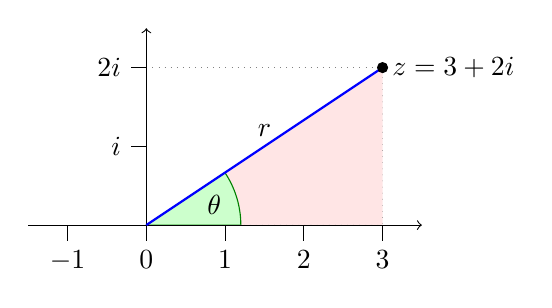
\begin{tikzpicture}
    \draw[help lines, dotted, fill=red!10] (0,0) -- (3,0) -- (3,2) -- cycle;
    \draw[help lines, dotted] (0,2) -- (3,2);
    \filldraw[fill=green!20,draw=green!50!black] (0,0) -- (1.2,0) arc (0:33.69:1.2) -- cycle;
    \node at (16.845:9mm){$\theta$};
    \draw[->](-1.5,0) -- (3.5,0);
    \draw[->](0,0) -- (0,2.5);
    \draw(0,1) -- +(-0.2,0) node[left] {$i$};
    \draw(0,2) -- +(-0.2,0) node[left] {$2i$};
    \draw(-1,0) -- +(0,-0.2) node[below] {$-1$};
    \draw(0,0) -- +(0,-0.2) node[below] {$0$};
    \draw(1,0) -- +(0,-0.2) node[below] {$1$};
    \draw(2,0) -- +(0,-0.2) node[below] {$2$};
    \draw(3,0) -- +(0,-0.2) node[below] {$3$};
    \draw[thick, blue] (0,0) -- node[above, black] {$r$} (3,2);
    \draw[fill, black] (3,2) circle [radius=1.8pt] node [right] {$z = 3+2i$};
  \end{tikzpicture}
\end{equation*}
The \textbf{magnitude}%
\index{complex number!magnitude}%
\index{magnitude!of a complex number} $r=\abs{z}$ of a complex number
is its distance from the origin. We also define the \textbf{argument}
of $z$ to be the angle $\theta$ between the $x$-axis and the line from
the origin to $z$, counted positively in the counterclockwise
direction. The magnitude $r$ and argument $\theta$ are shown in the
above picture.

Addition of complex numbers is like vector addition. The effect of
multiplying two complex numbers is to multiply their magnitudes and
add their arguments. For example, the following picture illustrates
the multiplication $(3+2i)(1+i)=1+5i$.
\begin{equation*}
  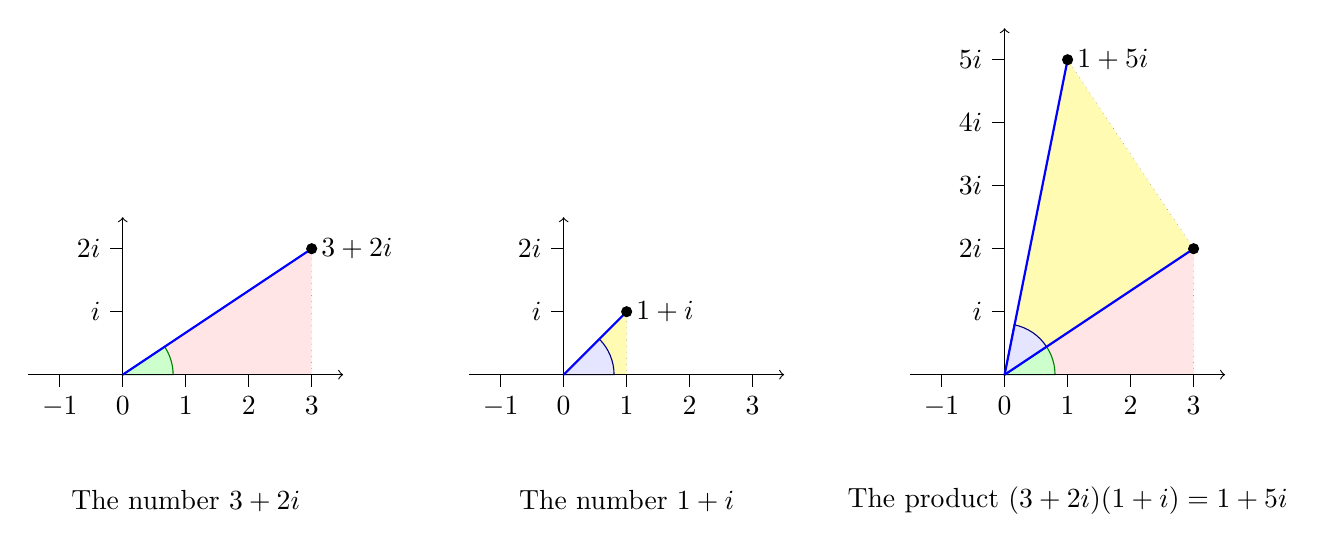
\begin{tikzpicture}[scale=0.8]
    \begin{scope}
      \draw[help lines, dotted, fill=red!10] (0,0) -- (3,0) -- (3,2) -- cycle;
      \filldraw[fill=green!20,draw=green!50!black] (0,0) -- (0.8,0) arc (0:33.69:0.8) -- cycle;
      \draw[->](-1.5,0) -- (3.5,0);
      \draw[->](0,0) -- (0,2.5);
      \draw(0,1) -- +(-0.2,0) node[left] {$i$};
      \draw(0,2) -- +(-0.2,0) node[left] {$2i$};
      \draw(-1,0) -- +(0,-0.2) node[below] {$-1$};
      \draw(0,0) -- +(0,-0.2) node[below] {$0$};
      \draw(1,0) -- +(0,-0.2) node[below] {$1$};
      \draw(2,0) -- +(0,-0.2) node[below] {$2$};
      \draw(3,0) -- +(0,-0.2) node[below] {$3$};
      \draw[thick, blue] (0,0) -- (3,2);
      \draw[fill, black] (3,2) circle [radius=2.25pt] node [right] {$3+2i$};
      \draw (1,-2) node {The number $3+2i$};
    \end{scope}
    \begin{scope}[xshift=7cm]
      \draw[help lines, dotted, fill=yellow!30] (0,0) -- (1,0) -- (1,1) -- cycle;
      \filldraw[fill=blue!10,draw=blue!50!black] (0,0) -- (0.8,0) arc (0:45:0.8) -- cycle;
      \draw[->](-1.5,0) -- (3.5,0);
      \draw[->](0,0) -- (0,2.5);
      \draw(0,1) -- +(-0.2,0) node[left] {$i$};
      \draw(0,2) -- +(-0.2,0) node[left] {$2i$};
      \draw(-1,0) -- +(0,-0.2) node[below] {$-1$};
      \draw(0,0) -- +(0,-0.2) node[below] {$0$};
      \draw(1,0) -- +(0,-0.2) node[below] {$1$};
      \draw(2,0) -- +(0,-0.2) node[below] {$2$};
      \draw(3,0) -- +(0,-0.2) node[below] {$3$};
      \draw[thick, blue] (0,0) -- (1,1);
      \draw[fill, black] (1,1) circle [radius=2.25pt] node [right] {$1+i$};
      \draw (1,-2) node {The number $1+i$};
    \end{scope}
    \begin{scope}[xshift=14cm]
      \draw[help lines, dotted, fill=red!10] (0,0) -- (3,0) -- (3,2) -- cycle;
      \draw[help lines, dotted, fill=yellow!30] (0,0) -- (3,2) -- (1,5) -- cycle;
      \filldraw[fill=green!20,draw=green!50!black] (0,0) -- (0.8,0) arc (0:33.69:0.8) -- cycle;
      \filldraw[fill=blue!10,draw=blue!50!black] (0,0) -- (33.69:0.8) arc (33:78.69:0.8) -- cycle;
      \draw[->](-1.5,0) -- (3.5,0);
      \draw[->](0,0) -- (0,5.5);
      \draw(0,1) -- +(-0.2,0) node[left] {$i$};
      \draw(0,2) -- +(-0.2,0) node[left] {$2i$};
      \draw(0,3) -- +(-0.2,0) node[left] {$3i$};
      \draw(0,4) -- +(-0.2,0) node[left] {$4i$};
      \draw(0,5) -- +(-0.2,0) node[left] {$5i$};
      \draw(-1,0) -- +(0,-0.2) node[below] {$-1$};
      \draw(0,0) -- +(0,-0.2) node[below] {$0$};
      \draw(1,0) -- +(0,-0.2) node[below] {$1$};
      \draw(2,0) -- +(0,-0.2) node[below] {$2$};
      \draw(3,0) -- +(0,-0.2) node[below] {$3$};
      \draw[thick, blue] (0,0) -- (3,2);
      \draw[fill, black] (3,2) circle [radius=2.25pt];
      \draw[thick, blue] (0,0) -- (1,5);
      \draw[fill, black] (1,5) circle [radius=2.25pt] node [right] {$1+5i$};
      \draw (1,-2) node {The product $(3+2i)(1+i)=1+5i$};
    \end{scope}
  \end{tikzpicture}
\end{equation*}
The effect of taking the complex conjugate is to reflect the given
complex number about the $x$ axis.
